% generated by scripts/pkl_to_latex.py
% source PKL : thermal_v1_L8_Ne8_U10_t1_mode-uniform_tpall_t2all_tperpall_nmin2_solver-gcg_full_restarts8_iter200_kmax4_tol1em09_cut10_adaptive1_step5_clusteravg1_T0to0.5_N20-3c87501b406b_knone_diag0.pkl
% scan type  : Tscan
% state      : gs
% x-max cap  : 0.5
% requires   : \usepackage{pgfplots} \pgfplotsset{compat=1.18}
% colours match the matplotlib PDF (tab10 cycle)
\definecolor{gmeC0}{HTML}{1F77B4}
\definecolor{gmeC1}{HTML}{FF7F0E}
\definecolor{gmeC2}{HTML}{2CA02C}
\definecolor{gmeC3}{HTML}{D62728}
\definecolor{gmeC4}{HTML}{9467BD}
\definecolor{gmeC5}{HTML}{8C564B}
\definecolor{gmeC6}{HTML}{E377C2}
\definecolor{gmeC7}{HTML}{17BECF}

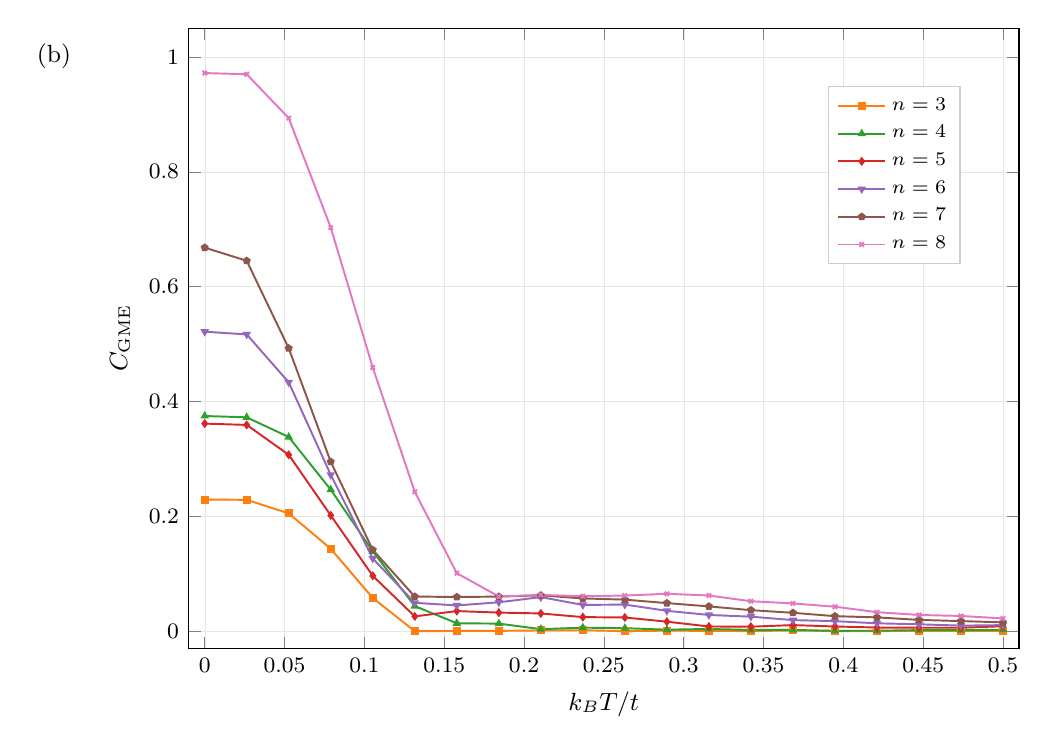
\begin{tikzpicture}
  \begin{axis}[
    width=\columnwidth,
    height=0.78\columnwidth,
    xlabel={$k_B T/t$},
    ylabel={$C_{\mathrm{GME}}$},
    grid=both,
    grid style={line width=.1pt, draw=gray!20},
    tick label style={font=\footnotesize\rmfamily, /pgf/number format/fixed},
    label style={font=\small\rmfamily},
    scaled ticks=false,
    legend style={font=\scriptsize\rmfamily, draw=gray!40, at={(0.5,1.03)}, anchor=south, /tikz/every even column/.append style={column sep=6pt}},
    legend cell align={left},
    legend columns=1,
    ymin=-0.03,
    ymax=1.05,
    xmin=-0.01,
    xmax=0.51,
    legend style={at={(0.850,0.763)}, anchor=center, fill=white},
    after end axis/.append code={\node[anchor=east, font=\small\rmfamily] at (axis description cs:-0.13,0.954) {(b)};},
  ]
    \addplot[color=gmeC1, mark=square*, mark size=1.1pt, line width=0.7pt] coordinates {
        (0,0.229253) (0.026316,0.228691) (0.052632,0.205165) (0.078947,0.143526)
        (0.105263,0.057789) (0.131579,0.000037) (0.157895,0.000338) (0.184211,0.000548)
        (0.210526,0.001244) (0.236842,0.001602) (0.263158,0.000044) (0.289474,0.00089)
        (0.315789,0.000491) (0.342105,0.000132) (0.368421,0.001237) (0.394737,0.000159)
        (0.421053,0.00007) (0.447368,0.000688) (0.473684,0.000261) (0.5,0.000286)
    };
    \addlegendentry{$n=3$}
    \addplot[color=gmeC2, mark=triangle*, mark size=1.1pt, line width=0.7pt] coordinates {
        (0,0.3747) (0.026316,0.37237) (0.052632,0.338121) (0.078947,0.24646)
        (0.105263,0.138824) (0.131579,0.043655) (0.157895,0.013756) (0.184211,0.013166)
        (0.210526,0.00353) (0.236842,0.006102) (0.263158,0.005214) (0.289474,0.002593)
        (0.315789,0.003868) (0.342105,0.002145) (0.368421,0.002172) (0.394737,0.000612)
        (0.421053,0.00082) (0.447368,0.001849) (0.473684,0.001656) (0.5,0.002536)
    };
    \addlegendentry{$n=4$}
    \addplot[color=gmeC3, mark=diamond*, mark size=1.1pt, line width=0.7pt] coordinates {
        (0,0.361429) (0.026316,0.35918) (0.052632,0.307082) (0.078947,0.201596)
        (0.105263,0.096367) (0.131579,0.02572) (0.157895,0.035015) (0.184211,0.032343)
        (0.210526,0.030864) (0.236842,0.024504) (0.263158,0.023828) (0.289474,0.016549)
        (0.315789,0.008178) (0.342105,0.007832) (0.368421,0.010597) (0.394737,0.008176)
        (0.421053,0.006316) (0.447368,0.006008) (0.473684,0.00595) (0.5,0.008613)
    };
    \addlegendentry{$n=5$}
    \addplot[color=gmeC4, mark=triangle*, mark size=1.1pt, mark options={rotate=180}, line width=0.7pt] coordinates {
        (0,0.521524) (0.026316,0.516758) (0.052632,0.433346) (0.078947,0.272261)
        (0.105263,0.126641) (0.131579,0.049413) (0.157895,0.044798) (0.184211,0.050308)
        (0.210526,0.059302) (0.236842,0.04569) (0.263158,0.046304) (0.289474,0.03547)
        (0.315789,0.028211) (0.342105,0.025274) (0.368421,0.019274) (0.394737,0.017431)
        (0.421053,0.01366) (0.447368,0.012015) (0.473684,0.009648) (0.5,0.010547)
    };
    \addlegendentry{$n=6$}
    \addplot[color=gmeC5, mark=pentagon*, mark size=1.1pt, line width=0.7pt] coordinates {
        (0,0.667932) (0.026316,0.644975) (0.052632,0.492598) (0.078947,0.294986)
        (0.105263,0.141515) (0.131579,0.060307) (0.157895,0.059489) (0.184211,0.06023)
        (0.210526,0.06233) (0.236842,0.057043) (0.263158,0.054932) (0.289474,0.048875)
        (0.315789,0.043138) (0.342105,0.036613) (0.368421,0.031973) (0.394737,0.026129)
        (0.421053,0.024022) (0.447368,0.019661) (0.473684,0.017553) (0.5,0.015331)
    };
    \addlegendentry{$n=7$}
    \addplot[color=gmeC6, mark=x, mark size=1.1pt, line width=0.7pt] coordinates {
        (0,0.97189) (0.026316,0.969891) (0.052632,0.893417) (0.078947,0.702852)
        (0.105263,0.459098) (0.131579,0.242702) (0.157895,0.101001) (0.184211,0.060397)
        (0.210526,0.063185) (0.236842,0.060766) (0.263158,0.062051) (0.289474,0.06511)
        (0.315789,0.062137) (0.342105,0.05213) (0.368421,0.048346) (0.394737,0.042601)
        (0.421053,0.03309) (0.447368,0.028233) (0.473684,0.026487) (0.5,0.022157)
    };
    \addlegendentry{$n=8$}
  \end{axis}
\end{tikzpicture}
